%!TEX program = xelatex
\documentclass{article}
\usepackage{amsthm,amsmath,amssymb}
\usepackage[UTF8]{ctex}
\usepackage[tc]{titlepic}
\usepackage{titlesec}
\usepackage{cite}
\usepackage{fancyhdr}
\usepackage{booktabs}
\usepackage{graphicx}
\usepackage{subfigure}
\usepackage{float}
\usepackage{geometry}
\usepackage[section]{placeins}
\usepackage{makeidx}
\usepackage{mathrsfs}
\usepackage{color}
\usepackage{ulem}
\usepackage{enumitem}
\everymath{\displaystyle}
\geometry{a4paper,scale=0.8}
\pagestyle{fancy}

\usepackage{hyperref}
\hypersetup{hypertex=true, colorlinks=true, linkcolor=blue, anchorcolor=blue, citecolor=blue}

\usepackage{listings}
\lstset{
    language=Python,
    basicstyle=\small\ttfamily,
    keywordstyle=\color{blue},
    commentstyle=\color{green},
    stringstyle=\color{red},
    showstringspaces=false,
    breaklines=true,
}

\lhead{第 2 次作业\\\today}
\chead{中国科学技术大学\\	DS4001 人工智能原理与技术}

\rhead{Homework 2\\ {\CTEXoptions[today=old]\today}}
\newcommand{\upcite}[1]{\textsuperscript{\cite{#1}}}

\titleformat*{\section}{\bfseries\Large}
\titleformat*{\subsection}{\bfseries\large}

\title{\bfseries 第二次作业(强化学习)}
\author{崔士强  \quad  PB22151743}

\begin{document}
\maketitle
\textcolor{red}{\textbf{本次作业需独立完成,不允许任何形式的抄袭行为,如被发现会有相应惩罚。在上方修改你的姓名学号,说明你同意本规定。}}
% \clearpage

\section*{问题1:热身(10分)}
\subsection*{a.计算(5分)}
\begin{table}[H]
    \centering
    \begin{tabular}{cccccc}
        \hline\hline
        $s$ & $-2$ & $-1$ & 0 & 1 & 2 \\
        \hline
        $V^{(0)}(s)$ & 0 & 0 & 0 & 0 & 0 \\
        $V^{(1)}(s)$ & 0 & 7.5 & $-10$ & 20 & 0 \\
        $V^{(2)}(s)$ & 0 & 2.5 & 5 & 16 & 0 \\
        \hline\hline
    \end{tabular}
\end{table}

\subsection*{b.计算(5分)}
\[\pi(s)=arg\ max_a\sum_{s' \in \mathcal{S}} \gamma P_{sas'} [R(s, a, s')+\gamma V(s')]\]
可以得到三个$(s, \mu(s))$数值对:$(-1, a_2), (0, a_1), (1, a_1)$


\section*{问题2:Q-Learning(15分)}
\subsection*{a.回答问题(2分)}
MDP具有时间齐性. $v(s)$和$q(s, a)$和状态转移概率有关,而状态转移概率不随时间变化而变化.

\subsection*{b.计算(8分)}
更新结果如下:
\begin{enumerate}
    \item $q(0, a_1)=2$
    \item $q(1, a_1)=1$
    \item $q(0, a_2)=-1$
    \item $q(1, a_1)=0$
\end{enumerate}

\subsection*{c.回答问题(5分)}
首先考虑Q函数与最大Q函数的差值. 由Bellman公式可以推导出,对一个状态-动作对,第n+1个Q函数最多是前一个的$\gamma$倍. 
而在每一个遍历区间,Q函数最大误差不超过$\gamma$倍的前一个最大误差,这样一来随着遍历区间数目的增长,最大误差趋近于零.


\section*{问题3:Gobang Programming(55分)}
\subsection*{a.回答问题(2分)}
由前面的分析过程,首先$Q^*$一定存在,因此经过足够多的迭代能够收敛. 再加上本例中状态空间并不大,应当可以在相对有限的轮数内收敛.

\subsection*{b.代码填空(33分)}
\begin{lstlisting}
class Gobang(UtilGobang):
    
    def get_next_state(self, action: Tuple[int, int, int], noise: Tuple[int, int, int]) -> np.array:

        # BEGIN_YOUR_CODE (our solution is 3 line of code, but don't worry if you deviate from this)
        next_state = self.board.copy()
        black, x_black, y_black = action
        next_state[x_black][y_black] = black
        # END_YOUR_CODE

        if noise is not None:
            white, x_white, y_white = noise
            next_state[x_white][y_white] = white
        return next_state

    def sample_noise(self) -> Union[Tuple[int, int, int], None]:

        if self.action_space:
            # BEGIN_YOUR_CODE (our solution is 2 line of code, but don't worry if you deviate from this)
            (x, y) = random.choice(self.action_space)
            self.action_space.remove((x, y))
            # END_YOUR_CODE
            return 2, x, y
        else:
            return None

    def get_connection_and_reward(self, action: Tuple[int, int, int],
                                  noise: Tuple[int, int, int]) -> Tuple[int, int, int, int, float]:

        # BEGIN_YOUR_CODE (our solution is 4 line of code, but don't worry if you deviate from this)
        (black_1, white_1) = self.count_max_connections(self.board)
        (black_2, white_2) = self.count_max_connections(self.get_next_state(action, noise))
        reward = pow(black_2, 2)-pow(white_2, 2)-pow(black_1, 2)+pow(white_1, 2)
        # END_YOUR_CODE

        return black_1, white_1, black_2, white_2, reward

    def sample_action_and_noise(self, eps: float) -> Tuple[Tuple[int, int, int], Tuple[int, int, int]]:

        # BEGIN_YOUR_CODE (our solution is 8 line of code, but don't worry if you deviate from this)
        state_hashable = self.array_to_hashable(self.board)
        
        if(random.random() < eps or state_hashable not in self.Q.keys()):
            action_ = random.choice(self.action_space)
            action = (1, action_[0], action_[1])
        else:
            actions = [(1, action[0], action[1]) for action in self.action_space if (1, action[0], action[1]) in self.Q[state_hashable].keys()]
            if(not actions):
                action_ = random.choice(self.action_space)
                action = (1, action_[0], action_[1])
            else:
                action = max(actions, key=self.Q[state_hashable].get)
        self.action_space.remove((action[1], action[2]))
        # END_YOUR_CODE
        return action, self.sample_noise()

    def q_learning_update(self, s0_: np.array, action: Tuple[int, int, int], s1_: np.array, reward: float,
                          alpha_0: float = 1):

        s0, s1 = self.array_to_hashable(s0_), self.array_to_hashable(s1_)
        self.s_a_visited[(s0, action)] = 1 if (s0, action) not in self.s_a_visited else \
            self.s_a_visited[(s0, action)] + 1
        alpha = alpha_0 / self.s_a_visited[(s0, action)]

        # BEGIN_YOUR_CODE (our solution is 18 line of code, but don't worry if you deviate from this)
        available_actions_s1 = [(1, action_[0], action_[1]) for action_ in self.action_space]
        have_Q = False
        for action_ in available_actions_s1:
            if s1 in self.Q.keys() and action_ in self.Q[s1].keys():
                have_Q = True
        if not have_Q :
            value_at_s1 = 0
        else:
            max_Q = -float("inf")
            for action_ in available_actions_s1:
                if(action_ not in self.Q[s1].keys()):
                    self.Q[s1][action_] = 0
                if(self.Q[s1][action_]>max_Q):
                    max_Q = self.Q[s1][action_]
            value_at_s1 = max_Q
        
        if(s0 not in self.Q.keys()):
            self.Q[s0] = {}
            self.Q[s0][action] = 0
        elif(action not in self.Q[s0].keys()):
            self.Q[s0][action] = 0
        self.Q[s0][action] -= alpha*(self.Q[s0][action]-reward-self.gamma*value_at_s1)
        # END_YOUR_CODE


\end{lstlisting}



\subsection*{c.结果复现(10分)}
\begin{figure}[H]
    \centering
    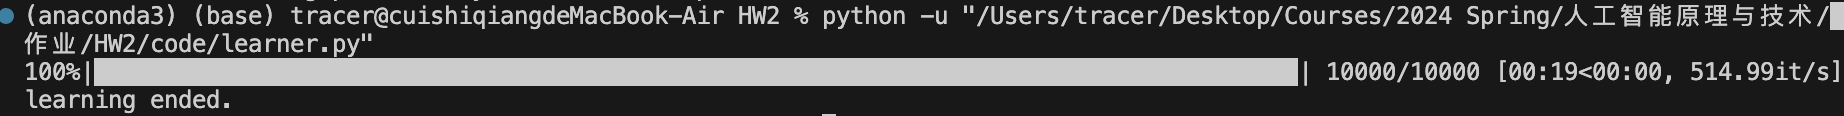
\includegraphics[width=15cm]{pics/3_train.png}
    \caption{训练结果}
\end{figure}
\begin{figure}[H]
    \centering
    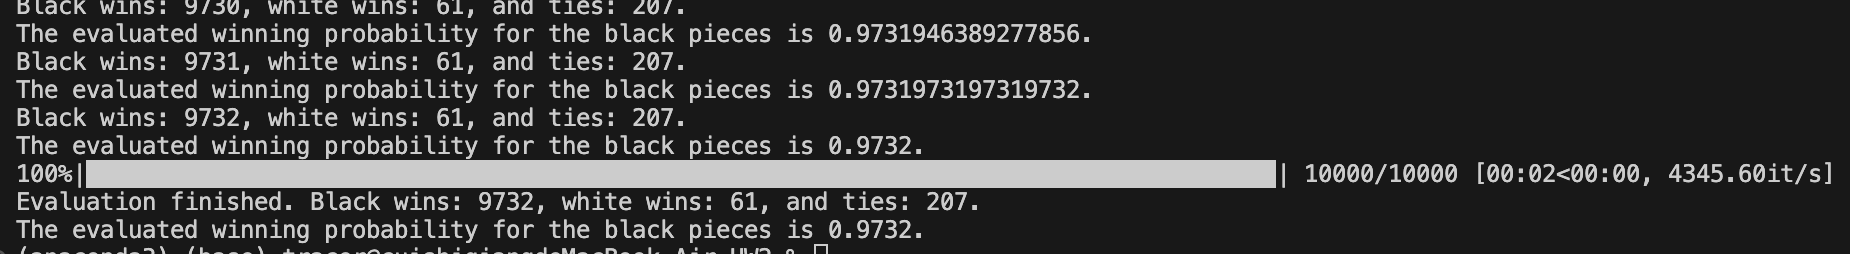
\includegraphics[width=15cm]{pics/3_eval.png}
    \caption{评估结果}
\end{figure}

\subsection*{d.回答问题(10分)}
\begin{figure}[H]
    \centering
    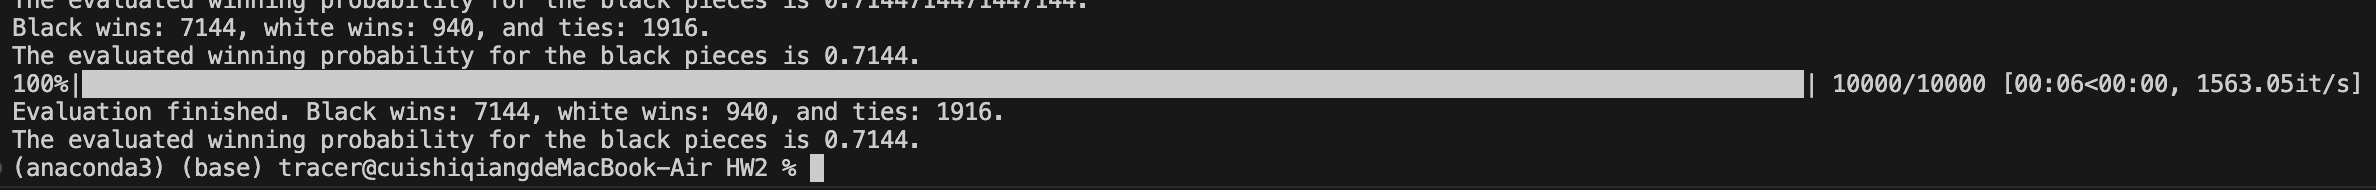
\includegraphics[width=15cm]{pics/4_eval_2.png}
    \caption{$n=4$的结果}
\end{figure}
该结果符合预期. 对于更大的状态和动作空间,遍历区间更长,收敛到$Q^*$更慢,所获取的$Q$函数离最优的距离更远,测试胜率更低.

\section*{问题4:Deeper Understanding(10分)}
\subsection*{a.回答问题(5分)}
\[\mathcal{T}_ \mu = \max_a \left(r_{sa}+ \gamma \cdot \sum_{s'\in\mathcal{S}} p_{sas'}\cdot v(s')\right)\]

\subsection*{b.回答问题(5分)}
由于概率之和为$1$,我们有
\[\sum_{s'\in\mathcal{S}} p_{sas'}\cdot v(s') \le \max_{s'\in\mathcal{S}}v(s')\]
因此
\[|\mathcal{T}_{v_1}(s)-\mathcal{T}_{v_2}(s)| \le \gamma \cdot \max_{s'\in\mathcal{S}}|v_1(s')-v_2(s')|\]
便可得到待证结论.


\section*{反馈(10分)}
% 在每次实验报告的最后欢迎反馈你上这门课的感受,你可以写下任何反馈,包括但不限于以下几个方面:课堂、作业难度和工作量、助教工作等等。

\begin{itemize}
    \item 本次作业相对第一次简单一些. 工作时间大约10h. 体验比较好.
    \item 另外由于不清楚赋值特性,不了解应当使用\lstinline|copy()|方法,导致debug时间很长.
\end{itemize}

\end{document}